\subsection{Gameplay UI}
\label{sec:UI_Gameplay}
The main interaction UI used throughout \ourgame{} will be placed at the bottom of the screen and will present options to the player character in bubbles. These bubbles will be context sensitive. In Figure~\ref{fig:UI_npc_talk}, the player is looking at an NPC, so the bubbles include the options described in Section~\ref{sec:conversation}. When the player is holding an item, the thought bubbles will include the options described in Section~\ref{sec:items}. Figure~\ref{fig:UI_npc_conversation} shows the UI during conversations. All of the UI representative of the player and their actions will be one hue, and all of the UI representative of other characters will be shown in a different hue.

\begin{figure}[htb]
  \centering\begin{subfigure}{.33\textwidth}
    \centering
    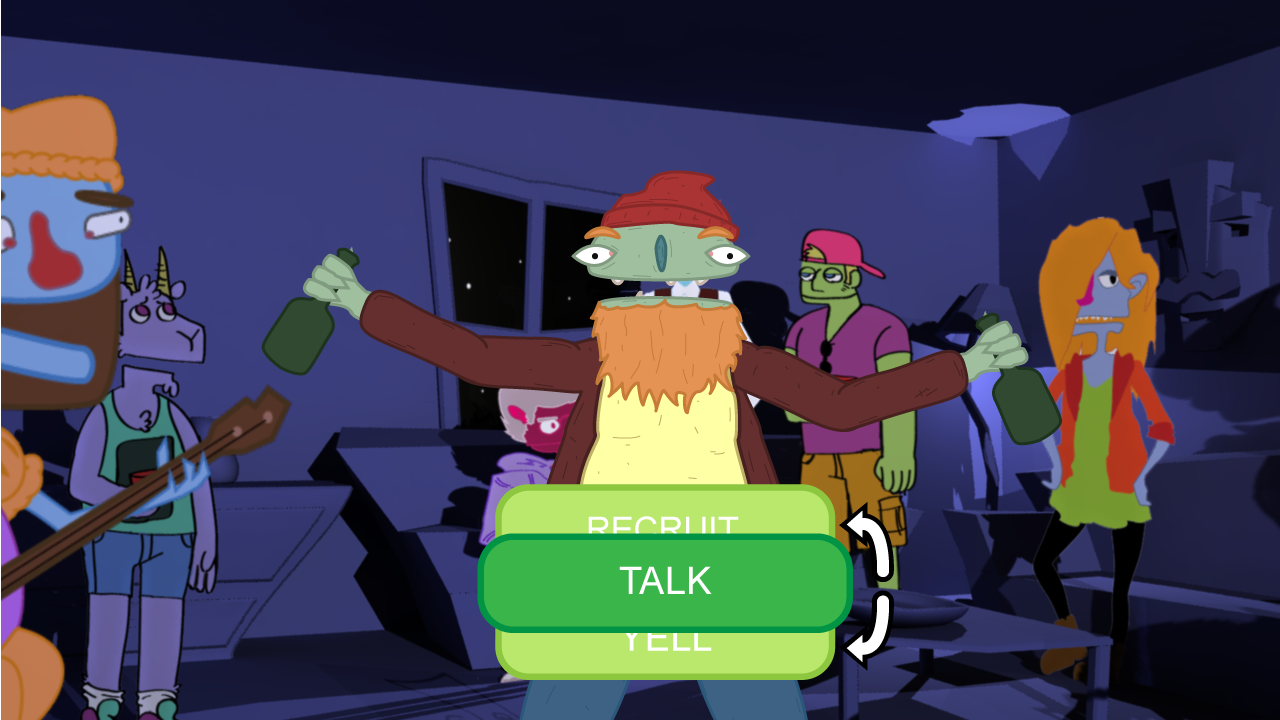
\includegraphics[width=.9\linewidth]{images/UI_npc_talk}
    \caption{NPC UI}
  	\label{fig:UI_npc_talk}
  \end{subfigure}%
  \begin{subfigure}{.33\textwidth}
    \centering
    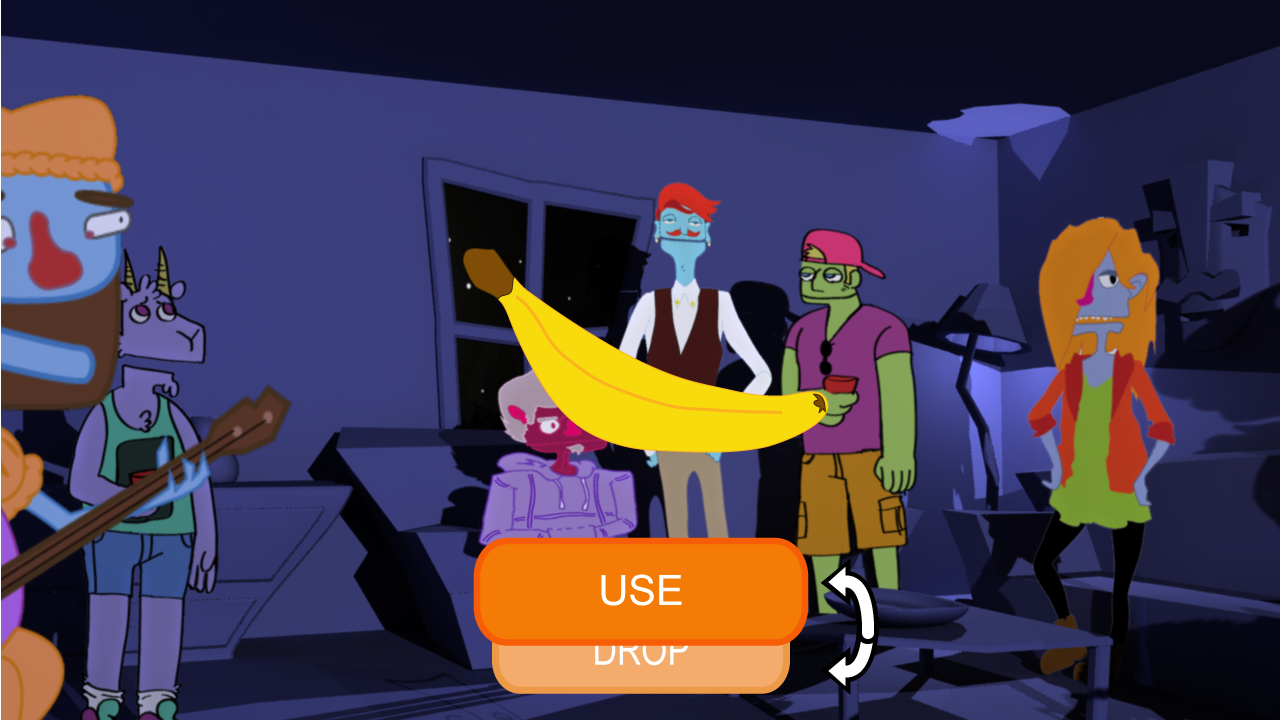
\includegraphics[width=.9\linewidth]{images/UI_item}
    \caption{Item UI}
  	\label{fig:UI_item}
  \end{subfigure}
  \begin{subfigure}{.33\textwidth}
    \centering
    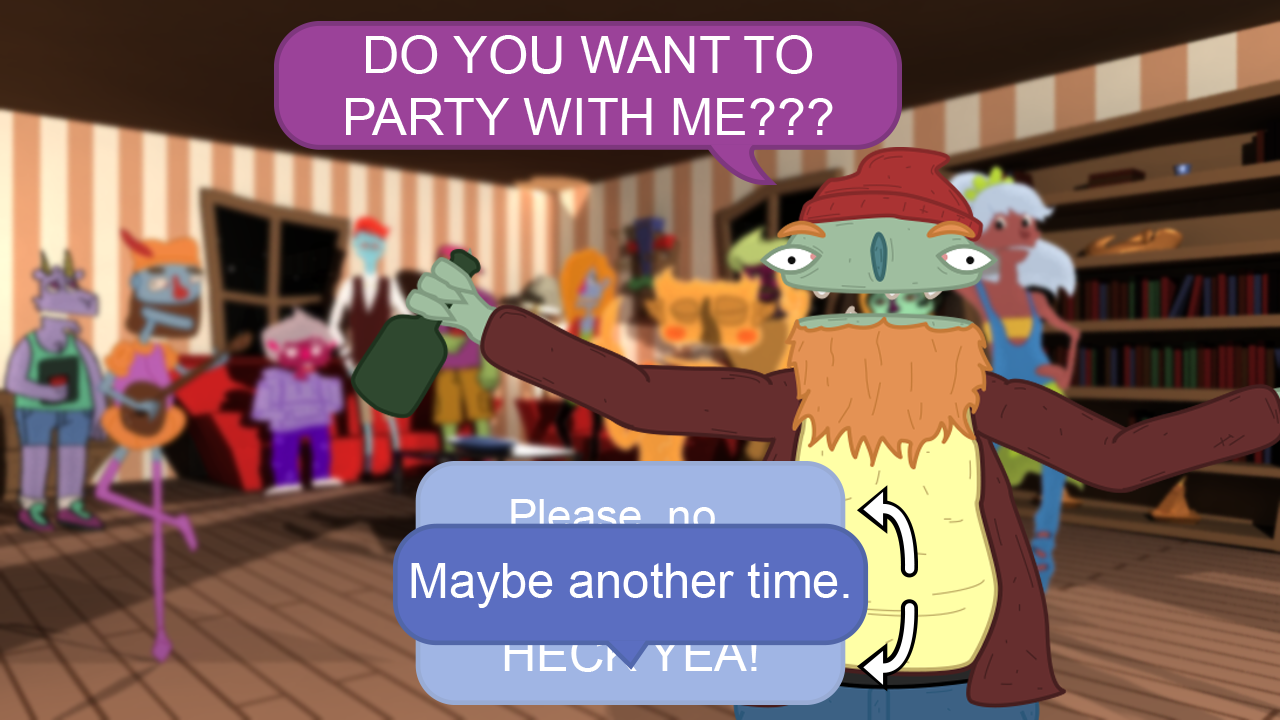
\includegraphics[width=.9\linewidth]{images/UI_npc_conversation}
    \caption{Conversation UI}
  	\label{fig:UI_npc_conversation}
  \end{subfigure}%
  \caption{Bubble interaction UI}
  \label{fig:gameplay_UI}
\end{figure}